% Created by tikzDevice version 0.10.1 on 2020-02-15 16:05:14
% !TEX encoding = UTF-8 Unicode
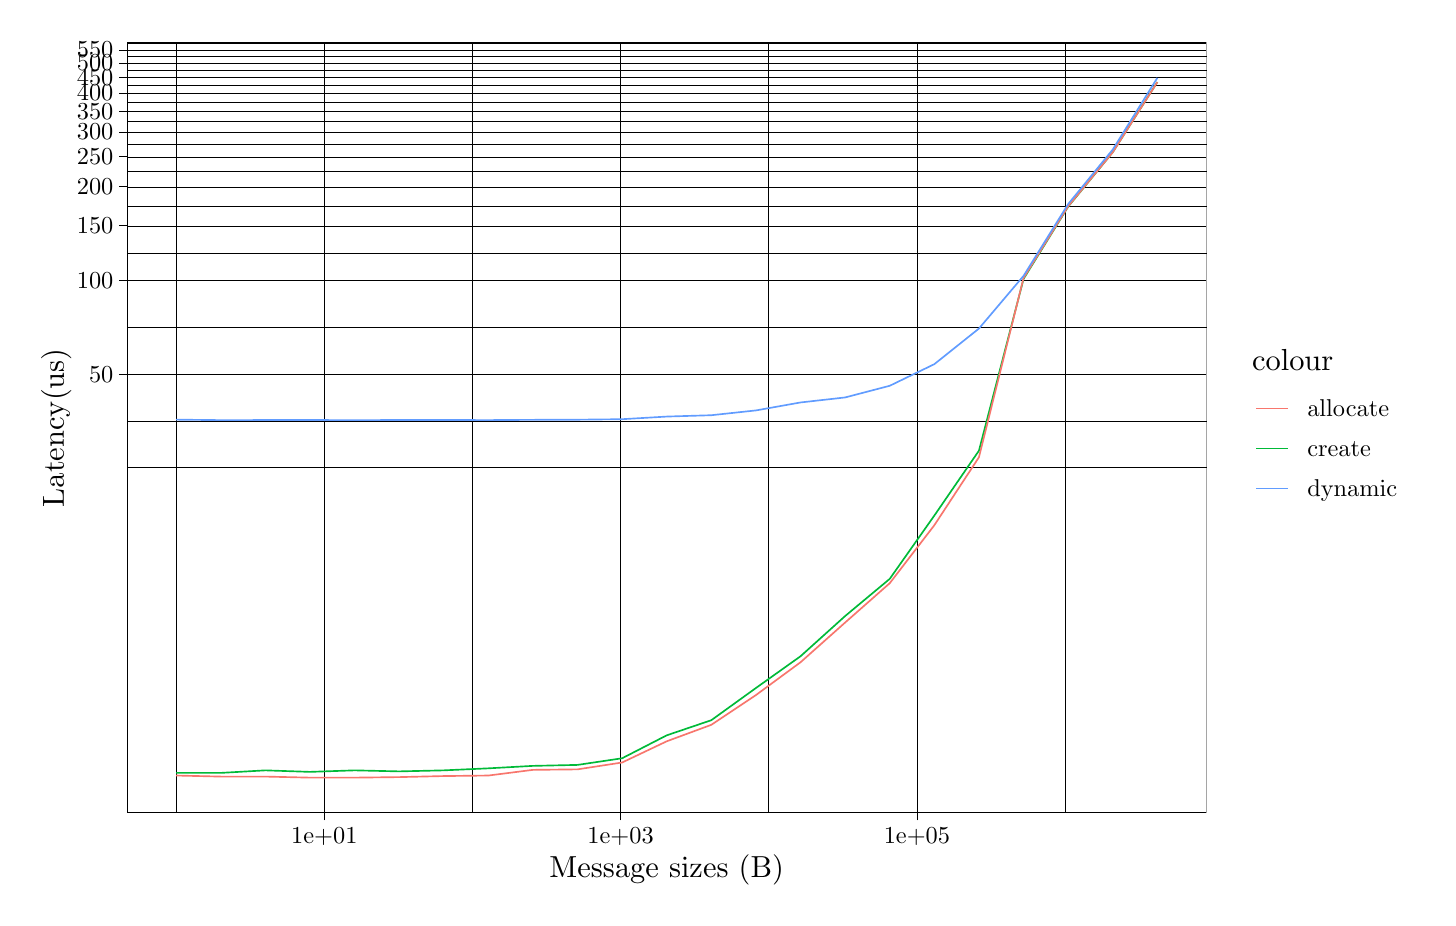
\begin{tikzpicture}[x=1pt,y=1pt]
\definecolor{fillColor}{RGB}{255,255,255}
\path[use as bounding box,fill=fillColor,fill opacity=0.00] (0,0) rectangle (505.89,314.37);
\begin{scope}
\path[clip] (  0.00,  0.00) rectangle (505.89,314.37);
\definecolor{drawColor}{RGB}{255,255,255}
\definecolor{fillColor}{RGB}{255,255,255}

\path[draw=drawColor,line width= 0.6pt,line join=round,line cap=round,fill=fillColor] (  0.00,  0.00) rectangle (505.89,314.37);
\end{scope}
\begin{scope}
\path[clip] ( 35.92, 30.72) rectangle (425.93,308.87);
\definecolor{fillColor}{RGB}{255,255,255}

\path[fill=fillColor] ( 35.92, 30.72) rectangle (425.93,308.87);
\definecolor{drawColor}{RGB}{0,0,0}

\path[draw=drawColor,line width= 0.0pt,line join=round] ( 35.92,155.27) --
	(425.93,155.27);

\path[draw=drawColor,line width= 0.0pt,line join=round] ( 35.92,172.20) --
	(425.93,172.20);

\path[draw=drawColor,line width= 0.0pt,line join=round] ( 35.92,206.06) --
	(425.93,206.06);

\path[draw=drawColor,line width= 0.0pt,line join=round] ( 35.92,232.89) --
	(425.93,232.89);

\path[draw=drawColor,line width= 0.0pt,line join=round] ( 35.92,249.82) --
	(425.93,249.82);

\path[draw=drawColor,line width= 0.0pt,line join=round] ( 35.92,262.30) --
	(425.93,262.30);

\path[draw=drawColor,line width= 0.0pt,line join=round] ( 35.92,272.21) --
	(425.93,272.21);

\path[draw=drawColor,line width= 0.0pt,line join=round] ( 35.92,280.42) --
	(425.93,280.42);

\path[draw=drawColor,line width= 0.0pt,line join=round] ( 35.92,287.45) --
	(425.93,287.45);

\path[draw=drawColor,line width= 0.0pt,line join=round] ( 35.92,293.59) --
	(425.93,293.59);

\path[draw=drawColor,line width= 0.0pt,line join=round] ( 35.92,299.04) --
	(425.93,299.04);

\path[draw=drawColor,line width= 0.0pt,line join=round] ( 35.92,303.94) --
	(425.93,303.94);

\path[draw=drawColor,line width= 0.0pt,line join=round] ( 53.64, 30.72) --
	( 53.64,308.87);

\path[draw=drawColor,line width= 0.0pt,line join=round] (160.72, 30.72) --
	(160.72,308.87);

\path[draw=drawColor,line width= 0.0pt,line join=round] (267.79, 30.72) --
	(267.79,308.87);

\path[draw=drawColor,line width= 0.0pt,line join=round] (374.87, 30.72) --
	(374.87,308.87);

\path[draw=drawColor,line width= 0.1pt,line join=round] ( 35.92,189.13) --
	(425.93,189.13);

\path[draw=drawColor,line width= 0.1pt,line join=round] ( 35.92,222.99) --
	(425.93,222.99);

\path[draw=drawColor,line width= 0.1pt,line join=round] ( 35.92,242.80) --
	(425.93,242.80);

\path[draw=drawColor,line width= 0.1pt,line join=round] ( 35.92,256.85) --
	(425.93,256.85);

\path[draw=drawColor,line width= 0.1pt,line join=round] ( 35.92,267.75) --
	(425.93,267.75);

\path[draw=drawColor,line width= 0.1pt,line join=round] ( 35.92,276.66) --
	(425.93,276.66);

\path[draw=drawColor,line width= 0.1pt,line join=round] ( 35.92,284.19) --
	(425.93,284.19);

\path[draw=drawColor,line width= 0.1pt,line join=round] ( 35.92,290.71) --
	(425.93,290.71);

\path[draw=drawColor,line width= 0.1pt,line join=round] ( 35.92,296.47) --
	(425.93,296.47);

\path[draw=drawColor,line width= 0.1pt,line join=round] ( 35.92,301.61) --
	(425.93,301.61);

\path[draw=drawColor,line width= 0.1pt,line join=round] ( 35.92,306.27) --
	(425.93,306.27);

\path[draw=drawColor,line width= 0.1pt,line join=round] (107.18, 30.72) --
	(107.18,308.87);

\path[draw=drawColor,line width= 0.1pt,line join=round] (214.26, 30.72) --
	(214.26,308.87);

\path[draw=drawColor,line width= 0.1pt,line join=round] (321.33, 30.72) --
	(321.33,308.87);
\definecolor{drawColor}{RGB}{0,186,56}

\path[draw=drawColor,line width= 0.6pt,line join=round] ( 53.64, 45.08) --
	( 69.76, 45.08) --
	( 85.88, 46.00) --
	(101.99, 45.45) --
	(118.11, 46.00) --
	(134.23, 45.63) --
	(150.34, 46.00) --
	(166.46, 46.73) --
	(182.58, 47.62) --
	(198.69, 47.97) --
	(214.81, 50.37) --
	(230.92, 58.66) --
	(247.04, 64.13) --
	(263.16, 75.76) --
	(279.27, 87.23) --
	(295.39,101.76) --
	(311.51,115.21) --
	(327.62,138.07) --
	(343.74,161.52) --
	(359.86,223.59) --
	(375.97,249.68) --
	(392.09,269.35) --
	(408.20,294.73);
\definecolor{drawColor}{RGB}{248,118,109}

\path[draw=drawColor,line width= 0.6pt,line join=round] ( 53.64, 44.13) --
	( 69.76, 43.75) --
	( 85.88, 43.75) --
	(101.99, 43.37) --
	(118.11, 43.37) --
	(134.23, 43.56) --
	(150.34, 43.94) --
	(166.46, 44.13) --
	(182.58, 46.18) --
	(198.69, 46.36) --
	(214.81, 48.84) --
	(230.92, 56.50) --
	(247.04, 62.46) --
	(263.16, 73.21) --
	(279.27, 85.06) --
	(295.39, 99.42) --
	(311.51,113.63) --
	(327.62,134.58) --
	(343.74,159.14) --
	(359.86,223.92) --
	(375.97,249.81) --
	(392.09,269.34) --
	(408.20,294.69);
\definecolor{drawColor}{RGB}{97,156,255}

\path[draw=drawColor,line width= 0.6pt,line join=round] ( 53.64,172.73) --
	( 69.76,172.55) --
	( 85.88,172.58) --
	(101.99,172.58) --
	(118.11,172.56) --
	(134.23,172.58) --
	(150.34,172.60) --
	(166.46,172.56) --
	(182.58,172.66) --
	(198.69,172.71) --
	(214.81,172.89) --
	(230.92,173.84) --
	(247.04,174.33) --
	(263.16,176.06) --
	(279.27,178.94) --
	(295.39,180.75) --
	(311.51,184.97) --
	(327.62,192.78) --
	(343.74,205.65) --
	(359.86,224.69) --
	(375.97,250.62) --
	(392.09,270.33) --
	(408.20,296.23);
\definecolor{drawColor}{RGB}{0,0,0}

\path[draw=drawColor,line width= 0.6pt,line join=round,line cap=round] ( 35.92, 30.72) rectangle (425.93,308.87);
\end{scope}
\begin{scope}
\path[clip] (  0.00,  0.00) rectangle (505.89,314.37);
\definecolor{drawColor}{RGB}{0,0,0}

\node[text=drawColor,anchor=base west,inner sep=0pt, outer sep=0pt, scale=  0.88] at ( 22.17,186.31) {50};

\node[text=drawColor,anchor=base west,inner sep=0pt, outer sep=0pt, scale=  0.88] at ( 17.77,220.17) {100};

\node[text=drawColor,anchor=base west,inner sep=0pt, outer sep=0pt, scale=  0.88] at ( 17.77,239.98) {150};

\node[text=drawColor,anchor=base west,inner sep=0pt, outer sep=0pt, scale=  0.88] at ( 17.77,254.03) {200};

\node[text=drawColor,anchor=base west,inner sep=0pt, outer sep=0pt, scale=  0.88] at ( 17.77,264.93) {250};

\node[text=drawColor,anchor=base west,inner sep=0pt, outer sep=0pt, scale=  0.88] at ( 17.77,273.84) {300};

\node[text=drawColor,anchor=base west,inner sep=0pt, outer sep=0pt, scale=  0.88] at ( 17.77,281.37) {350};

\node[text=drawColor,anchor=base west,inner sep=0pt, outer sep=0pt, scale=  0.88] at ( 17.77,287.89) {400};

\node[text=drawColor,anchor=base west,inner sep=0pt, outer sep=0pt, scale=  0.88] at ( 17.77,293.64) {450};

\node[text=drawColor,anchor=base west,inner sep=0pt, outer sep=0pt, scale=  0.88] at ( 17.77,298.79) {500};

\node[text=drawColor,anchor=base west,inner sep=0pt, outer sep=0pt, scale=  0.88] at ( 17.77,303.45) {550};
\end{scope}
\begin{scope}
\path[clip] (  0.00,  0.00) rectangle (505.89,314.37);
\definecolor{drawColor}{RGB}{0,0,0}

\path[draw=drawColor,line width= 0.3pt,line join=round] ( 33.17,189.13) --
	( 35.92,189.13);

\path[draw=drawColor,line width= 0.3pt,line join=round] ( 33.17,222.99) --
	( 35.92,222.99);

\path[draw=drawColor,line width= 0.3pt,line join=round] ( 33.17,242.80) --
	( 35.92,242.80);

\path[draw=drawColor,line width= 0.3pt,line join=round] ( 33.17,256.85) --
	( 35.92,256.85);

\path[draw=drawColor,line width= 0.3pt,line join=round] ( 33.17,267.75) --
	( 35.92,267.75);

\path[draw=drawColor,line width= 0.3pt,line join=round] ( 33.17,276.66) --
	( 35.92,276.66);

\path[draw=drawColor,line width= 0.3pt,line join=round] ( 33.17,284.19) --
	( 35.92,284.19);

\path[draw=drawColor,line width= 0.3pt,line join=round] ( 33.17,290.71) --
	( 35.92,290.71);

\path[draw=drawColor,line width= 0.3pt,line join=round] ( 33.17,296.47) --
	( 35.92,296.47);

\path[draw=drawColor,line width= 0.3pt,line join=round] ( 33.17,301.61) --
	( 35.92,301.61);

\path[draw=drawColor,line width= 0.3pt,line join=round] ( 33.17,306.27) --
	( 35.92,306.27);
\end{scope}
\begin{scope}
\path[clip] (  0.00,  0.00) rectangle (505.89,314.37);
\definecolor{drawColor}{RGB}{0,0,0}

\path[draw=drawColor,line width= 0.3pt,line join=round] (107.18, 27.97) --
	(107.18, 30.72);

\path[draw=drawColor,line width= 0.3pt,line join=round] (214.26, 27.97) --
	(214.26, 30.72);

\path[draw=drawColor,line width= 0.3pt,line join=round] (321.33, 27.97) --
	(321.33, 30.72);
\end{scope}
\begin{scope}
\path[clip] (  0.00,  0.00) rectangle (505.89,314.37);
\definecolor{drawColor}{RGB}{0,0,0}

\node[text=drawColor,anchor=base,inner sep=0pt, outer sep=0pt, scale=  0.88] at (107.18, 19.71) {1e+01};

\node[text=drawColor,anchor=base,inner sep=0pt, outer sep=0pt, scale=  0.88] at (214.26, 19.71) {1e+03};

\node[text=drawColor,anchor=base,inner sep=0pt, outer sep=0pt, scale=  0.88] at (321.33, 19.71) {1e+05};
\end{scope}
\begin{scope}
\path[clip] (  0.00,  0.00) rectangle (505.89,314.37);
\definecolor{drawColor}{RGB}{0,0,0}

\node[text=drawColor,anchor=base,inner sep=0pt, outer sep=0pt, scale=  1.10] at (230.92,  7.44) {Message sizes (B)};
\end{scope}
\begin{scope}
\path[clip] (  0.00,  0.00) rectangle (505.89,314.37);
\definecolor{drawColor}{RGB}{0,0,0}

\node[text=drawColor,rotate= 90.00,anchor=base,inner sep=0pt, outer sep=0pt, scale=  1.10] at ( 13.08,169.80) {Latency(us)};
\end{scope}
\begin{scope}
\path[clip] (  0.00,  0.00) rectangle (505.89,314.37);
\definecolor{fillColor}{RGB}{255,255,255}

\path[fill=fillColor] (436.93,135.11) rectangle (500.39,204.49);
\end{scope}
\begin{scope}
\path[clip] (  0.00,  0.00) rectangle (505.89,314.37);
\definecolor{drawColor}{RGB}{0,0,0}

\node[text=drawColor,anchor=base west,inner sep=0pt, outer sep=0pt, scale=  1.10] at (442.43,190.44) {colour};
\end{scope}
\begin{scope}
\path[clip] (  0.00,  0.00) rectangle (505.89,314.37);
\definecolor{fillColor}{RGB}{255,255,255}

\path[fill=fillColor] (442.43,169.52) rectangle (456.89,183.97);
\end{scope}
\begin{scope}
\path[clip] (  0.00,  0.00) rectangle (505.89,314.37);
\definecolor{drawColor}{RGB}{248,118,109}

\path[draw=drawColor,line width= 0.6pt,line join=round] (443.88,176.74) -- (455.44,176.74);
\end{scope}
\begin{scope}
\path[clip] (  0.00,  0.00) rectangle (505.89,314.37);
\definecolor{drawColor}{RGB}{248,118,109}

\path[draw=drawColor,line width= 0.6pt,line join=round] (443.88,176.74) -- (455.44,176.74);
\end{scope}
\begin{scope}
\path[clip] (  0.00,  0.00) rectangle (505.89,314.37);
\definecolor{drawColor}{RGB}{248,118,109}

\path[draw=drawColor,line width= 0.6pt,line join=round] (443.88,176.74) -- (455.44,176.74);
\end{scope}
\begin{scope}
\path[clip] (  0.00,  0.00) rectangle (505.89,314.37);
\definecolor{fillColor}{RGB}{255,255,255}

\path[fill=fillColor] (442.43,155.06) rectangle (456.89,169.52);
\end{scope}
\begin{scope}
\path[clip] (  0.00,  0.00) rectangle (505.89,314.37);
\definecolor{drawColor}{RGB}{0,186,56}

\path[draw=drawColor,line width= 0.6pt,line join=round] (443.88,162.29) -- (455.44,162.29);
\end{scope}
\begin{scope}
\path[clip] (  0.00,  0.00) rectangle (505.89,314.37);
\definecolor{drawColor}{RGB}{0,186,56}

\path[draw=drawColor,line width= 0.6pt,line join=round] (443.88,162.29) -- (455.44,162.29);
\end{scope}
\begin{scope}
\path[clip] (  0.00,  0.00) rectangle (505.89,314.37);
\definecolor{drawColor}{RGB}{0,186,56}

\path[draw=drawColor,line width= 0.6pt,line join=round] (443.88,162.29) -- (455.44,162.29);
\end{scope}
\begin{scope}
\path[clip] (  0.00,  0.00) rectangle (505.89,314.37);
\definecolor{fillColor}{RGB}{255,255,255}

\path[fill=fillColor] (442.43,140.61) rectangle (456.89,155.06);
\end{scope}
\begin{scope}
\path[clip] (  0.00,  0.00) rectangle (505.89,314.37);
\definecolor{drawColor}{RGB}{97,156,255}

\path[draw=drawColor,line width= 0.6pt,line join=round] (443.88,147.84) -- (455.44,147.84);
\end{scope}
\begin{scope}
\path[clip] (  0.00,  0.00) rectangle (505.89,314.37);
\definecolor{drawColor}{RGB}{97,156,255}

\path[draw=drawColor,line width= 0.6pt,line join=round] (443.88,147.84) -- (455.44,147.84);
\end{scope}
\begin{scope}
\path[clip] (  0.00,  0.00) rectangle (505.89,314.37);
\definecolor{drawColor}{RGB}{97,156,255}

\path[draw=drawColor,line width= 0.6pt,line join=round] (443.88,147.84) -- (455.44,147.84);
\end{scope}
\begin{scope}
\path[clip] (  0.00,  0.00) rectangle (505.89,314.37);
\definecolor{drawColor}{RGB}{0,0,0}

\node[text=drawColor,anchor=base west,inner sep=0pt, outer sep=0pt, scale=  0.88] at (462.39,173.71) {allocate};
\end{scope}
\begin{scope}
\path[clip] (  0.00,  0.00) rectangle (505.89,314.37);
\definecolor{drawColor}{RGB}{0,0,0}

\node[text=drawColor,anchor=base west,inner sep=0pt, outer sep=0pt, scale=  0.88] at (462.39,159.26) {create};
\end{scope}
\begin{scope}
\path[clip] (  0.00,  0.00) rectangle (505.89,314.37);
\definecolor{drawColor}{RGB}{0,0,0}

\node[text=drawColor,anchor=base west,inner sep=0pt, outer sep=0pt, scale=  0.88] at (462.39,144.81) {dynamic};
\end{scope}
\end{tikzpicture}
